\section{Step 1 - The frame}
\label{SectionStep1}
Our first step is to provide a frame which is used in the next steps.
This frame consists of a menu where we can hook functions to be selected and a canvas where all our drawings will be displayed.

Read and run {\tt Step1.py} (see listing~\ref{LISTING_STEP1_PY} given below)
\footnote{In the following sections only the relevant parts of the code is presented in the script.
If you are not sure how this code fits into the program please read the example code listing.}.

Figure~\ref{STEP_1_SCREEN} shows what you should get if you execute {\tt Step1.py}.
If you installed all what's needed you should see our empty pythonOCC screen.
Please study the code and the comments added.
If you have questions don't worry.
The comments in the code provide more information than needed for following this step by step course.
If you just accept the code as it is and try to figure out how to get something similar done that's fine for the moment.

It is interesting to note that there is no import of a GUI-framework like {\tt import~wx} in the code.
All the GUI stuff is found in {\tt OCC.Display.SimpleGui}.
In that module the environment is examined and the approprate GUI framework is initalized.
So if you like to know what is going on behind the scene have a look at {\tt OCC.Display.SimpleGui}\footnote{If you make use of wxPython you can also use the sample given in Appendix~\ref{Appendix_wx_PySimpleApp}. Here a sample of the appilcation of the class {wx.PySimpleApp} is given.}.

% +++++++++++++++++++++++++++++++++++++++++++++++++++++++++++++++++++++++ 
% +++ Bild: Step 1 ++++++++++++++++++++++++++++++++++++++++++++++++++++++
% +++++++++++++++++++++++++++++++++++++++++++++++++++++++++++++++++++++++ 
\begin{figure}[h]
\begin{center}
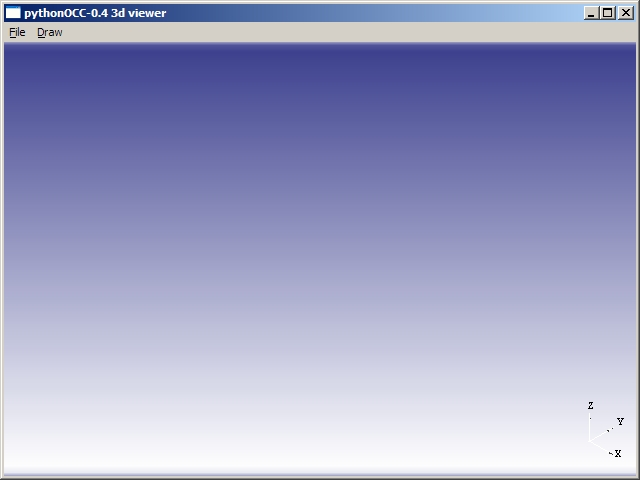
\includegraphics[height=8.5cm,width=11.3cm]{Step1.jpg}
\end{center}
\caption[Screenshot of Step1]{\label{STEP_1_SCREEN}Screenshot of Step1}
\end{figure}

\pagebreak
\begin{python}[moreemph={[4], 46, 48},caption={Step1.py - The program frame},label=LISTING_STEP1_PY]
# =============================================================================
# Packages to import
# =============================================================================
import sys
from OCC.Display.SimpleGui import * 
# =============================================================================
# Functions called from some menu-items
# =============================================================================
def draw_nothing(event=None):
    pass

def exit(event=None):
    sys.exit()
# =============================================================================
# Main-part: If this script is running as a main script, i.e. it 
# is directly called by Python the following is executed.
# =============================================================================
if __name__ == '__main__':
    # OCC.Display.SimpleGui.init_display() returns multiple
    # values which are assigned here
    display, start_display, add_menu, add_function_to_menu = \
        init_display()
    # This is the place where we hook our functionality to menus
    # ----------------------------------------------------------
    add_menu('File')
    add_function_to_menu('File',  exit)
    add_menu('Draw')
    add_function_to_menu('Draw', draw_nothing)
    
    start_display()
\end{python}

That's the frame so get ready to add some geometry.
